% --------------------------------------------------------------------------- %
%            _       _                 _            _   _                     %
%           (_)_ __ | |_ _ __ ___   __| |_   _  ___| |_(_) ___  _ __          %
%           | | '_ \| __| '__/ _ \ / _` | | | |/ __| __| |/ _ \| '_ \         %
%           | | | | | |_| | | (_) | (_| | |_| | (__| |_| | (_) | | | |        %
%           |_|_| |_|\__|_|  \___/ \__,_|\__,_|\___|\__|_|\___/|_| |_|        %
% --------------------------------------------------------------------------- %
\chapter{Towards Sound ARt Composition and Performance}
\label{sec: introduction}
\epigraph{\emph{Music, which should pulsate with life, needs new means of expression, and science alone can infuse it with youthful vigor.}}{\citep{varese1966}}

\begin{figure}
    \centering
    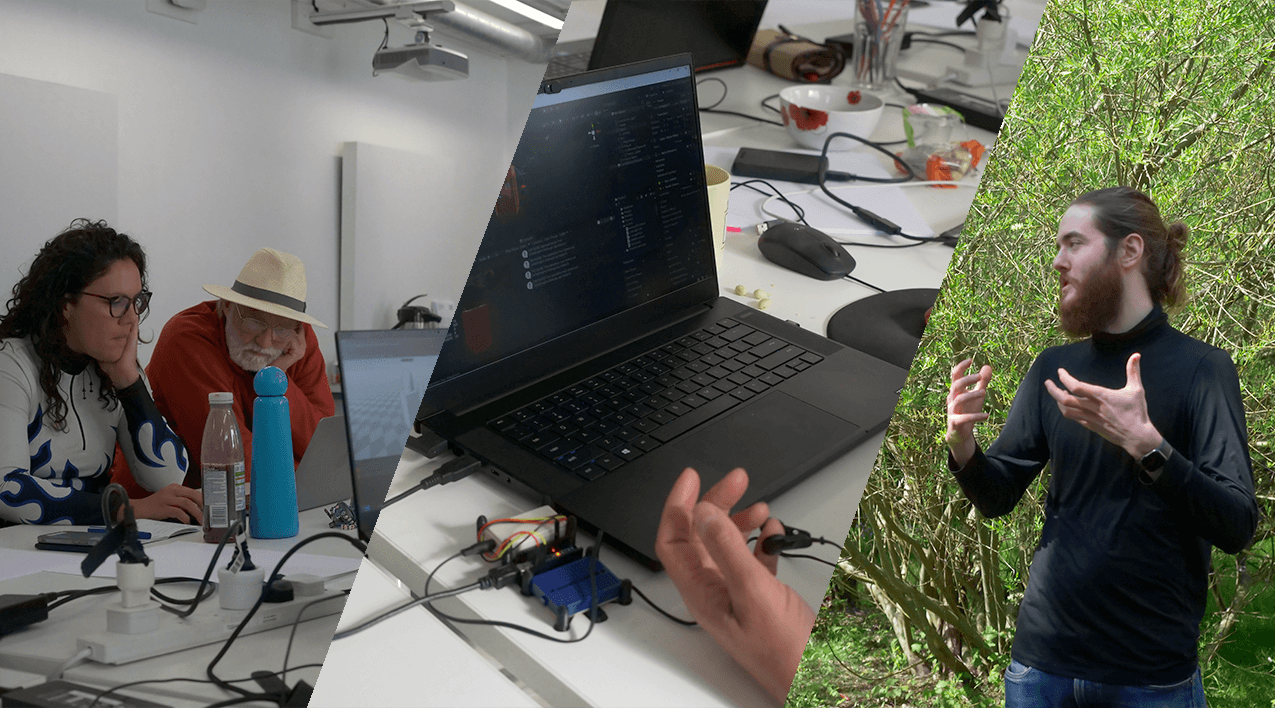
\includegraphics[width=1\linewidth]{01-intro/chapter-fig.png}
    \captionsetup{labelformat=empty}
    \caption[\autoref*{sec: introduction}'s page-figure: \textit{polygons\textasciitilde{}} in performance at the Attenborough Centre for Creative Arts, University of Sussex, on June 8th, (from \citeauthor{bilbow2022a}, \citeyear{bilbow2022a})]{}
\end{figure}

\clearpage
% --------------------------------------------------------------------------- %
\section{Summary}\label{sec: introduction-summary}

In the last twenty years, computational technology has become more and more expressive, the systems we engage with becoming increasingly interactive. Due to this, the arts, including forms of digital sound art, have embraced new technologies in tandem with, and often contributing to, their development. This has led to more human-centred methods of designing tools of digital art creation, moving away from black-boxed (undisclosed to the audience) interactions, towards more performative and suggestive interactions, which often include the audience. Among some of the technologies that have seen nascent use in the arts is \gls{xr} \footnote{The meaning of `X' in \gls{xr} is a hotly contested topic, check its term entry for more on its definition}, a group of technologies that promise to radically rethink the way we approach digital and physical reality. 

The category of \gls{xr} is comprised of: \gls{vr} - technology that promises to immerse us in a completely synthetic virtual world; and \gls{ar} - technology that promises to immerse us in our own real world through the computational mediation of virtual processes \footnote{The present thesis makes no distinction between the modern usage of the term \gls{mr} and that of \gls{ar}. Although commendable for being process-agnostic (i.e. mixed, not limited to augmentation), this thesis aligns itself with the larger body of academic research and creative practice that uses the term \gls{ar}}. This leads to the augmentation, diminution, hybridisation, or extension of our own experience of reality, blurring and perhaps dissolving the line between our virtual and real selves.

\gls{ar}, as mentioned, has seen sporadic use in the arts in the last twenty years. Its use in other disciplines, such as medical science, manufacturing and repair, annotation and visualisation, and the military \citep{azuma1997}, have been typically characterised by its use as technology that aids or facilitates the \textbf{visual overlay and alignment} of \textbf{virtual graphics} (text, image, animation, video) onto our \textbf{real world environment}. Within these fields, this has a potential myriad important uses, from training junior doctors in dummy procedures by overlaying the steps of a difficult surgery, to allowing three-dimensional networked collaboration across vast distances. Within the arts, its use has also been typically limited to this `visual overlay' approach. Despite being only a fraction of the possible forms of \gls{ar}, this conception of \gls{ar} dominates the market of consumer \gls{ar} devices, from head-mounted, to handheld and projective technologies, the majority deal with overlaying visual information. 

By taking a \gls{diy} approach to designing and implementing custom digital musical tools through hardware and software in \autoref{sec: method}, the present practice-based research thesis approaches \gls{ar} through a multisensory lens to designing rich, expressive experience. The importance of such an approach is in its ability help redefine, and understand more about the technologies with which we are choosing to mediate our daily lives with, considering their origins, and also about how our own perception of digital media is affected through this embodied usage.


% --------------------------------------------------------------------------- %
\section{Personal Motivations}\label{sec: introduction-motivations}
My own motivations for taking this approach to \gls{ar} experience is in the potential for it to afford creative, rich, sensory artwork, which seeks to teach us more about the way we perceive ourselves, others, and our environment. Coming from a background in music technology, specifically in developing and evaluating digital music tools and instruments, the nature of typical `visual overlay' \gls{ar} is seemingly incompatible with its use as a digital music tool. As such, it seems not only possible, but reasonable for it to be redefined to encapsulate all senses, and processes of perceptual modulation. In wanting to foster embodied experience between audience members (collaborative expression), \gls{ar} offers a unique way of mediating and co-constructing the space in which they embody. Thus, my motivation is also within the advancement of our understanding this hybrid space-time, in which unique relationships between virtual and real processes are played out.

Real space, and increasingly virtual space, due to their pervasiveness and entanglement with the body, are inherently political media; substrates that we are all suspended in to different degrees, with their currents systemically shaped by those with political power or access to capital. They have and increasingly are being used to marginalise and commit violence against specific groups of people, through architecture, and through media. This thesis adopts my politics of being a green socialist, anti-racist, and feminist. Although it is by no means a political commentary, these positions are important to raise when outlining the rationale and motivation for the current work. As well as being a tool for violence and marginalisation, space, and specifically technologically mediated forms of space, can provide the foundation for radical acts of political expression through art.

Over the last three years, the NIME and sound art practice community has increasingly integrated \gls{xr} into its toolset for \gls{dmi} design, evaluation, composition, and performance \citep[e.g.][]{chevalier2017,lee2020,camci2021}. Crucially, this comes at a time when corporations actively vie for a monopoly on virtual space, and by extension, our digitally mediated lives. Tangential to the questions outlined below, one of the main themes of the thesis is the accessibility, affordability, and sustainability of the digital tools used in sound art practice. This theme invariably involves the aforementioned anti-capitalist position, and thus aims where possible to reduce the amount of consumer technology used, in favour of \gls{diy} and Maker approaches.



% --------------------------------------------------------------------------- %
\section{Key Research Questions}\label{sec: introduction-researchquestions}
As outlined, \gls{ar} has seen nascent implementation as a creative medium in the arts, and more specifically music composition and performance. Therefore, the research areas and questions for the present thesis are based in the intersection between the arts, technology, sensory perception:

\RQall

% --------------------------------------------------------------------------- %
\section{Aims \& Objectives of the Thesis}\label{sec: introduction-aims}
As well as answering and contributing understanding to the above research questions, this thesis aims to:

\begin{itemize}
    \item Conduct a thorough literature and practice review of the field of \gls{ar} generally and within the arts
    \item Apply theories of materiality, embodiment, and space to contemporary \gls{ar} design, use, and evaluation.
    \item Contribute to the practice field of \gls{ar} sound arts by designing and evaluating \gls{ar} experiences for creative and collaborative expression.
    \item Contribute to the understanding of how such tools might affect our perceptions of self, others and our real, virtual, and hybrid environments. 
    \item Propose workflows that may help artists and musicians interested in leveraging \gls{ar} within sound art composition and performance
\end{itemize}



% --------------------------------------------------------------------------- %
\section{Research Methods}\label{sec: introduction-methods}
The research methods used to answer my research questions, and achieve my aims and objectives above involve taking a practice-based approach to designing multisensory digital musical instruments using \gls{ar}. Much of this is grounded in a resistance to the origin of \gls{ar} from within the U.S. \gls{mic}, and the effects this has had on the typical form of \gls{ar} found today, explored in \autoref{sec: ar-arts}, and \autoref{sec: method}. In developing three sound \gls{art} experiences, which were qualitatively evaluated through autobiographical design, and grounded theory coded interviews, I iteratively redesigned them to provide rich and immersive experience to myself as well as participants and audiences. This iteration has led to a set of reproducible design guidelines for artists and musicians interested in using \gls{ar} creatively in \autoref{sec: discussion-guidelines}, as well as theoretical implications for the sonic medium found in \autoref{sec: conclusion}.




% --------------------------------------------------------------------------- %
\section{Outline of Chapters}\label{sec: introduction-outline}
\autoref{sec: review} starts with a review of \gls{ar} as an emerging technology within the field of \gls{hci}, examining the effects that historical barriers to usage such as portability, price, as well as its origination in the \gls{mic}, have had on typical forms today. Among these forms, it is found that the majority deal with simple and descriptive visual additions in the form of text, image, animation or video overlay. I make a case for `multisensory' \gls{ar}, i.e. the designing of content or experience for multiple senses to counter not only this bias toward visual design, but also as a method of attaining richer and more novel experiences of \gls{ar}. This case is made by examining current advancements in multisensory \gls{hci} applications and enabling technologies. In the second part of the chapter, I posit through a review of contemporary art practice, the potential of \gls{ar} use within the arts in contributing to the designing and evaluation of expressive tools, enabling new aesthetic and multisensory experiences, collaborative expression, and agency.

In \autoref{sec: theory}, I outline the position that the thesis takes regarding aesthetic experience and artistic production, as well as outlining a key contemporary theory of cognition: \gls{4ec}, that may help explicate aesthetic experience in \gls{ar}. I identify three lenses through which to view, not only the potential of modern-day applications of sound \gls{art}, but also the potential of the medium itself. The first is through a consideration of the \textbf{materiality} and form of complex processes in \glspl{dmi} and interactive music systems for designers, performer, and audience. The second is through examining of current theories of enactivism and \textbf{embodied} action within \gls{xr} technologies. The last is through considering the intervention of \gls{ar} processes in real and virtual \textbf{spaces}, how this effects the construction of these spaces, the implications this in-turn has for the type of art that is created, and the privacy and security of people co-located in these spaces - is the Metaverse really where we want our \gls{art} to exist and be `consumed'? 

\autoref{sec: method} contains the methodology through which I address my research questions, this is separated into three sections. First, I contextualise the methodological approach taken within the findings of the previous two chapters. Secondly, an outlining of the concept of resistance, which has guided and motivated my practical and theoretical work towards \glsfirst{opensource} technologies, non-visual sensory displays, and the processual nature of \gls{ar}'s ability to modulate perception. Thirdly, I examine individually the methods taken in the ensuing three study chapters.
 
In \autoref{sec: area}, I outline the development and evaluation of the \textit{area\textasciitilde{}} system. \textit{area\textasciitilde{}} enables users to record, manipulate, and spatialise virtual audio samples or nodes around their immediate environment. Through a combination of ambisonics audio rendering and hand gesture tracking, this system calls attention to the ability of non-visual \gls{ar}, here, \gls{aar}, to provide new aesthetic experiences of real and virtual environments. Through an \gls{abd} study, this pilot study proposes that rich experience can result from non-visual \gls{ar} systems. 

\autoref{sec: polaris} describes the design, experience, and evaluation of an \gls{av} \gls{ar} piece called {polaris\textasciitilde{}}, developed using mainly \gls{floss} and \gls{osh}. Studies took place in October 2021, and the experiences of 10 participants were analysed using the grounded theory analysis method to draw out commonalities. In evaluating \textit{polaris\textasciitilde{}} it was found that the experience engaged participants fruitfully, with many noting their ability to express themselves audiovisually in creative ways. The remarks from the transcriptions of these studies, that were then sorted into the categories of Sentiment, Learning, Adoption, Expression, and Immersion. 

\autoref{sec: polygons} outlines my journey deploying \gls{ar} as a tool for sound \gls{art} performance, detailing problems, solutions, and the experience of performing the piece \textit{polygons\textasciitilde{}} in \gls{ar}. The performance was the first time I had immersed myself in the \textit{polygons\textasciitilde{}} system for an extended period of time which lead to an authentic exploration and improvisation of the material, embodied, and spatial affordances of the three instruments in the system \textit{ambi}, \textit{click+-}, and \textit{hands}.

\autoref{sec: discussion} briefly reviews the position of the thesis as carved out in \autoref{sec: review} and \autoref{sec: theory}, before discussing the \gls{diy} method outlined in \autoref{sec: method}. Combined results of the three studies are highlighted, and I propose a set of design guidelines through which artists and musicians in the field can produce expressive works using \gls{ar}. The thesis is concluded in \autoref{sec: conclusion} with a review of contributions, a set of implications for the sonic medium of \gls{ar}, as well as future recommendations.

\section{VR as a Medium for Computational Art and Music}
A parallel field to the one explored in this thesis is that of \gls{vr} as a medium for computational art and musical expression. \gls{vr}, which has benefited from being a long-term focus of fields such as telerobotics, entertainment (mainly gaming), has been explored much more thoroughly in the \gls{nime} field. The distinction between \gls{vr} and \gls{ar}, as outlined in the beginning of this chapter, is the location of user immersion - either in a virtual world, or in the real world respectively. Currently, this makes a great impact on its mode of usage within the context of an artistic work, and therefore renders \gls{vr} outside the scope of this thesis for the time being. Readers interested in the use of \gls{vr} as a medium for musical composition and performance are advised to consult the recent publication: `Sonic Interactions in Virtual Environments', which provides a comprehensive overview of the field \citep{geronazzo2023}. Of particular interest to the themes explored in this thesis are the following of its chapters: 

\begin{itemize}
    \item Spatial Design Considerations for Interactive Audio in Virtual Reality - \citep{deacon2023}
    \item Embodied and Sonic Interactions in Virtual Environments: Tactics and Exemplars - \citep{olsen2023}
    \item Supporting Sonic Interaction in Creative, Shared Virtual Environments - \citep{men2023}
    \item Audio in Multisensory Interactions: From Experiments to Experiences - \citep{serafin2023}
    \item From the Lab to the Stage: Practical Considerations on Designing Performances with Immersive Virtual Musical Instruments - \citep{zappi2023}
\end{itemize}

\section{Contributions}\label{sec: intro-contrib}
The contributions to knowledge of the present research cover four main areas, material, methodological, theoretical, and communal, and are as follows:
\begin{SingleSpace}
    \subsubsection{Material}
        \begin{noitemize}
            \item The \textit{\hyperref[sec: area]{\textit{area\textasciitilde{}}}} \gls{aar} compositional tool. Patch and schematics are available online. 
            \item The \textit{\hyperref[sec: polaris]{\textit{polaris\textasciitilde{}}}} \gls{av} \gls{ar} experience. Code and patches are \glshyperlink[open-source]{opensource}.
            \item The \textit{\hyperref[sec: polygons]{\textit{polygons\textasciitilde{}}}} \gls{av} \gls{ar} performance system. Code and patches are \glshyperlink[open-source]{opensource}.
            \item Design \href{https://github.com/AheadIO/Deck-X/tree/main/Deck_X/STL_files/Headgear/Welding_Headgear_Adaptor}{contributions} to the accessibility of the \gls{pns} headset.
        \end{noitemize}
\subsubsection{Methodological}
    \begin{noitemize}
        \item Presentation of \textit{area\textasciitilde{}} at International Conference on Auditory Displays (ICAD) 2020 \href{https://icad.org/abba-august-2020/}{`Auditory Brown Bag at Home'} series, and the Interact Conference 2021 \href{https://youtu.be/IQPof8-esM0?t=1690}{`Multisensory Augmented Reality'} workshop \citep[evaluated in][]{bilbow2021a}.
        \item Presentation of research at Tangible, Embedded, and Embodied Interaction (TEI) 2021 \href{https://www.youtube.com/watch?v=zyO43URZZDk}{`Graduate Student Consortium'} \citep[outlined in][]{bilbow2021b}.
        \item Presentation of \textit{polaris\textasciitilde{}} at New Interfaces for Musical Expression (NIME) 2022 \href{https://www.youtube.com/watch?v=eCdQku5hFOE}{`Mixed \& Augmented Reality'} paper session \citep[evaluated in][]{bilbow2022}
        \item Presentation on \glshyperlink[open-source]{opensource} \gls{ar} for the \href{https://www.youtube.com/watch?v=A826j_RwxeA}{CodeDay} non-profit organisation.
    \end{noitemize}
    \subsubsection{Theoretical}
    \begin{noitemize}
        \item Proposal of \textit{`augmented materiality'}, \textit{`augmented embodiment'}, and \textit{`augmented space'} (\autoref{sec: conclusion}).
        \item Design Guidelines for Sound \gls{art} (\autoref{sec: discussion-guidelines}).
        \item Co-authored position paper on \gls{4ec} within sound \gls{art} \citep{bilbow2021}.
    \end{noitemize}
\subsubsection{Communal}
    \begin{noitemize}
        \item Performances and demos of \textit{polygons\textasciitilde{}} \citep{bilbow2022b,bilbow2022a}
        \item Peer-reviewed a paper on \gls{mr} for Tangible, Embedded, and Embodied Interaction (TEI) conference.
        \item Creation and maintenance of `The XRt Space' \href{https://sambilbow.github.io/thexrtspace}{website} and \href{https://discord.gg/p3MmURSBV3}{Discord server}.
        \item Co-development and administration of the `Arts Research Community' (ARC) \href{https://discord.gg/8dfsZDgwN8}{Discord server} at Sussex University. 
        \item Co-facilitation of the Embodiment Hackathon at Sussex University \citep{bonarjee2022}.
        \item Co-facilitation of the Leverhulme Sussex \href{https://www.sussex.ac.uk/sensation/training/seminars}{Seminar Series}.
        \item Co-facilitation of the Leverhulme Sensation Sussex \href{https://www.sussex.ac.uk/sensation/training/conference-2021}{Conference 2021}.
    \end{noitemize}
\end{SingleSpace}




